\chapter{Evaluation}\label{chap:evaluation}
Once the problem is set and the data is prepared,  machine learning model is applied to solve the problem. But, The model built to solve the problem might not be good, lot of time is spend on choosing, running and tuning algorithms. One way to test the machine learning model is to, define the test harness on which the model performance can be computed. Another method is, compare the the model by adding more input samples. 

In this research, two models are built, one for the detection of migration and one for the detection of sentiment. Evaluation of sentiment detection model is discussed in Section \ref{snetimentdetectionmodel}. The migration detection model's performance metrics is discussed in the Section \ref{migration_detection_experiment}. In addition to these evaluation metrics, the migration model is evaluated by adding more samples that are not considered from the data collection step but from the other external source. Hereinafter, the new samples is called as canadian migration dataset. The technique is discussed in the section \ref{eval}. combined data is preprocessd with same series of step which was discused in Section \ref{preprocessing} . The model is built using this data with three classifier algorithm. 

The distribution of tweets after combining migration dataset and canadian migration dataset is shown in the graph \ref{fig:combined}. The confusion matrix of all the three classifier is given the table [\ref{tab:confusionmatrix_migrationtweets_com_LR},\ref{tab:confusionmatrix_migrationtweets_com_NB},\ref{tab:confusionmatrix_migrationtweets_com_DT}] and the performance metric is given the table \ref{tab:sentiment_metric_com}.

Comparing the two metric table  \ref{tab:sentiment_metric_com} and \ref{tab:Migration_metric}


\begin{figure}
	\centering
	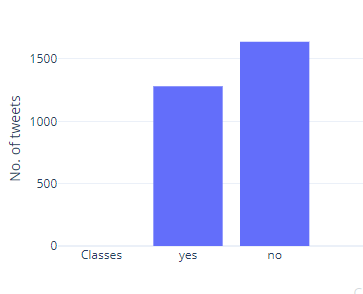
\includegraphics[width=10cm\linewidth,height=10cm]{thesis_template/images/combined.png}
	\caption{Distribution of the combined tweets}
	\label{fig:combined}
\end{figure}




\begin{table}[]
\centering
\begin{tabular}{lllll}
\cline{1-3}
\multicolumn{1}{|l|}{}   & \multicolumn{1}{l|}{predicted\_YES} & \multicolumn{1}{l|}{predicted\_NO}  &  &  \\ \cline{1-3}
\multicolumn{1}{|l|}{YES} & \multicolumn{1}{l|}{158}  & \multicolumn{1}{l|}{81} &  &  \\ \cline{1-3}
\multicolumn{1}{|l|}{NO}   & \multicolumn{1}{l|}{52}  & \multicolumn{1}{l|}{234}  &  &  \\ \cline{1-3}
                            &                           &                           &  & 
\end{tabular}
\caption{Logistic regression:Confusion matrix for migration model on combined dataset}
\label{tab:confusionmatrix_migrationtweets_com_LR}
\end{table}

\begin{table}[]
\centering
\begin{tabular}{lllll}
\cline{1-3}
\multicolumn{1}{|l|}{}   & \multicolumn{1}{l|}{predicted\_YES} & \multicolumn{1}{l|}{predicted\_NO}  &  &  \\ \cline{1-3}
\multicolumn{1}{|l|}{YES} & \multicolumn{1}{l|}{166}  & \multicolumn{1}{l|}{73} &  &  \\ \cline{1-3}
\multicolumn{1}{|l|}{NO}   & \multicolumn{1}{l|}{100}  & \multicolumn{1}{l|}{186}  &  &  \\ \cline{1-3}
                            &                           &                           &  & 
\end{tabular}
\caption{Niave Bayes: Confusion matrix for migration model on combined dataset}
\label{tab:confusionmatrix_migrationtweets_com_NB}
\end{table}


\begin{table}[]
\centering
\begin{tabular}{lllll}
\cline{1-3}
\multicolumn{1}{|l|}{}   & \multicolumn{1}{l|}{predicted\_YES} & \multicolumn{1}{l|}{predicted\_NO}  &  &  \\ \cline{1-3}
\multicolumn{1}{|l|}{YES} & \multicolumn{1}{l|}{170}  & \multicolumn{1}{l|}{69} &  &  \\ \cline{1-3}
\multicolumn{1}{|l|}{NO}   & \multicolumn{1}{l|}{70}  & \multicolumn{1}{l|}{216}  &  &  \\ \cline{1-3}
                            &                           &                           &  & 
\end{tabular}
\caption{Decision trees: Confusion matrix for migration model on combined dataset}
\label{tab:confusionmatrix_migrationtweets_com_DT}
\end{table}

\begin{table}[]
\centering
\begin{tabular}{lllll}
\hline
\textbf{Classifier} & \textbf{Accuracy} & \textbf{Precision} & \textbf{Recall} & \textbf{F1-score} \\ \hline
Logistic regression & 0.746           & 0.752              & 0.661           & 0.703            \\ \hline
Naive Bayes         & 0.670             & 0.624              & 0.694           & 0.657             \\ \hline
Decision Trees     & 0.735             & 0.708              & 0.711           & 0.709             \\ \hline
\end{tabular}
\caption{Performance metric of all the classifier - Migration model on combined dataset}
\label{tab:sentiment_metric_com}
\end{table}


